\documentclass[12pt]{article}
 
\usepackage[margin=1in]{geometry} 
\usepackage{amsmath,amsthm,amssymb}
\usepackage{graphicx}
\usepackage{float}
\usepackage{tikz}
\usetikzlibrary{arrows,shapes,trees} % loads some tikz extensions
 
\begin{document}
 
\title{Homework 4}
\author{Josh Klontz
CSE 802}
 
\maketitle

\begin{enumerate}
\item \textbf{Consider the following data drawn from two distributions in two dimensions.}
\begin{enumerate}
\item \textbf{Compute the sample means.}
\begin{equation}
\begin{split}
m_1& = (-3.6, -1.2) \\
m_2& = (2.6, 0.4)
\end{split}
\end{equation}
\item \textbf{Compute the within-class scatter matrix.}
\begin{figure}[H]
\begin{verbatim}
function [ Si ] = scatter(x)
    mi = mean(x);
    Si = zeros(length(mi), length(mi));
    for i=1:length(x),
        Si = Si + transpose(x(i,:)-mi) * (x(i,:) - mi);
    end
end
\end{verbatim}
\caption{MATLAB code to compute a scatter matrix.}
\end{figure}
\begin{equation}
S_w = \left[ \begin{array}{cc} 70.4 & 10.2 \\ 10.2 & 56 \end{array} \right]
\end{equation}
\item \textbf{Compute the between-class scatter matrix.}
\begin{equation}
S_b = \left[ \begin{array}{cc} 38.44 & 9.92 \\ 9.92 & 2.56 \end{array} \right]
\end{equation}
\item \textbf{Find the Fisher Linear Discriminant for this data.}
\begin{equation}
\text{Fisher Linear Discriminant} = (-0.0862, -0.0129)
\end{equation}
\item \textbf{Plot the data points and the discriminant.}
\begin{figure}[H]
\centering
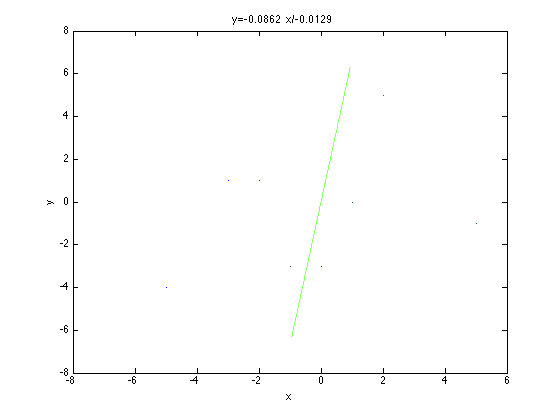
\includegraphics[width=4in]{1}
\caption{The points and the discriminant.}
\end{figure}
\end{enumerate}
\item \textbf{Face Recognition!}
\begin{enumerate}
\item \textbf{Align the face images based on the location of the
eyes and resize them.} \\
Completed using OpenBR: \texttt{br -algorithm RegisterFace -enroll FERET\_100 FERET\_100\_registered}
\item \textbf{Calculate the set of top 100 Eigenfaces and Fisherfaces; visualize
the top 20 basis faces to see what they look like.}
\begin{figure}[H]
\begin{verbatim}
function [ data ] = loadData(path)
    files = dir(path);
    files = files(3:length(files)); % remove '.' and '..'
    rows = numel(imread(strcat(path,'/',files(1).name())));
    columns = length(files);
    data = zeros(rows, columns);
    for i=1:length(files),
        data(:,i) = reshape(imread(strcat(path,'/',files(i).name())), rows, 1);    
    end
end
\end{verbatim}
\caption{MATLAB code to read training data.}
\end{figure}
\begin{figure}[H]
\begin{verbatim}
function [m vecs vals] = pca(data)
    m = zeros(size(data,1),1);
    for i=1:size(data,1),
        m(i) = mean(data(i,:));
    end
    for i=1:size(data,2),
        data(:,i) = data(:,i)-m;
    end
    scatter = transpose(data)*data;
    [vecs vals] = eig(scatter);
    vecs = data * vecs;
end
\end{verbatim}
\caption{MATLAB code for PCA.}
\end{figure}
\begin{figure}[H]
\begin{verbatim}
function [m vecs vals] = lda(data)
    numClasses = 100;
    numSamples = 5;
    
    [pcaM, pcaVecs] = pca(data);
    pcaVecs = pcaVecs(:,numClasses+1:size(data,2));
    data = transpose(pcaVecs)*(data-repmat(pcaM,1,size(data,2)));
    
    d = size(data,1);
    m = zeros(d,1);
    Sw = zeros(d,d);
    Sb = zeros(d,d);
    for i=1:size(data,1),
        m(i) = mean(data(i,:));
    end
    
    for i=0:numClasses-1,
        mi = zeros(d,1);
        for j=1:d,
            mi(j) = mean(data(j,i*numSamples+1:(i+1)*numSamples));
        end
        for j=1:numSamples,
            delta = data(:,i*numSamples+j)-mi;
            Sw = Sw + delta * transpose(delta);
        end
        delta = mi - m;
        Sb = Sb + numSamples * (delta * transpose(delta));
    end
    [vecs vals] = eig(Sb, Sw);
    vecs = pcaVecs * vecs;
end
\end{verbatim}
\caption{MATLAB code for LDA.}
\end{figure}
\begin{figure}[H]
\begin{verbatim}
function [] = visualize(vectors, path)
    n = min(size(vectors,2), 20);
    for i=0:n-1,
        m = reshape(vectors(:,size(vectors,2)-i), 128, 96);
        m = m - min(min(m));
        m = m ./ max(max(m));
        imwrite(m, strcat(path,'/',int2str(i),'.png'));
    end
end
\end{verbatim}
\caption{MATLAB code for visualizing eigenvectors.}
\end{figure}
\begin{table}[H]
\centering
\begin{tabular}{ccccc}
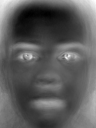
\includegraphics[width=1in]{pca/0}&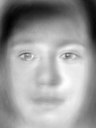
\includegraphics[width=1in]{pca/1}&
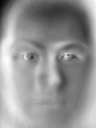
\includegraphics[width=1in]{pca/2}&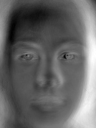
\includegraphics[width=1in]{pca/3}&
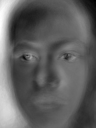
\includegraphics[width=1in]{pca/4}\\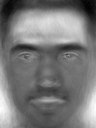
\includegraphics[width=1in]{pca/5}&
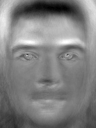
\includegraphics[width=1in]{pca/6}&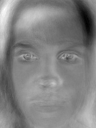
\includegraphics[width=1in]{pca/7}&
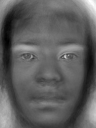
\includegraphics[width=1in]{pca/8}&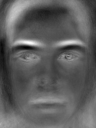
\includegraphics[width=1in]{pca/9}\\
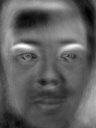
\includegraphics[width=1in]{pca/10}&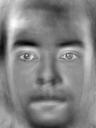
\includegraphics[width=1in]{pca/11}&
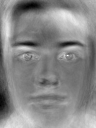
\includegraphics[width=1in]{pca/12}&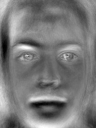
\includegraphics[width=1in]{pca/13}&
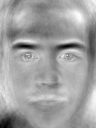
\includegraphics[width=1in]{pca/14}\\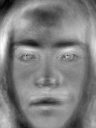
\includegraphics[width=1in]{pca/15}&
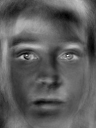
\includegraphics[width=1in]{pca/16}&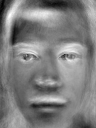
\includegraphics[width=1in]{pca/17}&
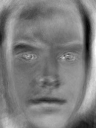
\includegraphics[width=1in]{pca/18}&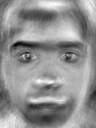
\includegraphics[width=1in]{pca/19}\\
\end{tabular}
\caption{Top 20 Eigenfaces.}
\end{table}
\begin{table}[H]
\centering
\begin{tabular}{ccccc}
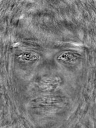
\includegraphics[width=1in]{lda/0}&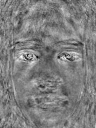
\includegraphics[width=1in]{lda/1}&
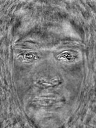
\includegraphics[width=1in]{lda/2}&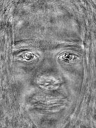
\includegraphics[width=1in]{lda/3}&
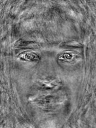
\includegraphics[width=1in]{lda/4}\\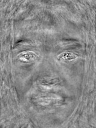
\includegraphics[width=1in]{lda/5}&
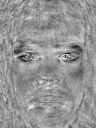
\includegraphics[width=1in]{lda/6}&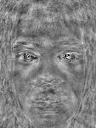
\includegraphics[width=1in]{lda/7}&
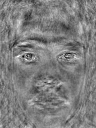
\includegraphics[width=1in]{lda/8}&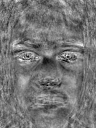
\includegraphics[width=1in]{lda/9}\\
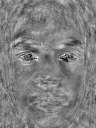
\includegraphics[width=1in]{lda/10}&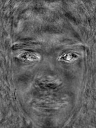
\includegraphics[width=1in]{lda/11}&
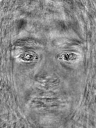
\includegraphics[width=1in]{lda/12}&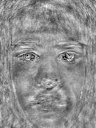
\includegraphics[width=1in]{lda/13}&
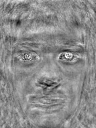
\includegraphics[width=1in]{lda/14}\\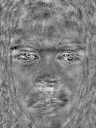
\includegraphics[width=1in]{lda/15}&
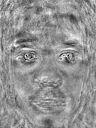
\includegraphics[width=1in]{lda/16}&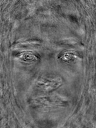
\includegraphics[width=1in]{lda/17}&
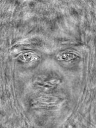
\includegraphics[width=1in]{lda/18}&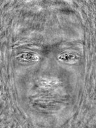
\includegraphics[width=1in]{lda/19}\\
\end{tabular}
\caption{Top 20 Fisherfaces.}
\end{table}
\item \textbf{Capture 10 images of your own face and 10 images of five of your
friends using your mobile phone camera.}
\begin{table}[H]
\centering
\begin{tabular}{cccccc}
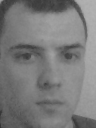
\includegraphics[width=1in]{test/0-0}&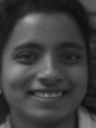
\includegraphics[width=1in]{test/1-0}&
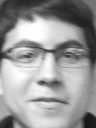
\includegraphics[width=1in]{test/2-0}&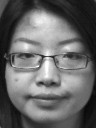
\includegraphics[width=1in]{test/3-0}&
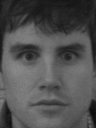
\includegraphics[width=1in]{test/4-0}&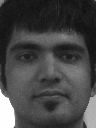
\includegraphics[width=1in]{test/5-0}\\
\end{tabular}
\caption{Acquired faces.}
\end{table}
\item \textbf{Represent the faces in (c) in terms of Eigenfaces and Fisherfaces; show the reconstruction ability as the number of basis faces are increased.}
\begin{table}[H]
\centering
\begin{tabular}{cccc}
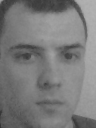
\includegraphics[width=1in]{test/0-0}&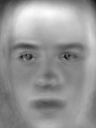
\includegraphics[width=1in]{reconstruct/0}&
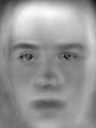
\includegraphics[width=1in]{reconstruct/1}&\includegraphics[width=1in]{reconstruct/2}\\
\end{tabular}
\caption{Reconstructed face with 1, 10, and 100 eigenvectors.}
\end{table}
\item \textbf{Determine the error rate of the nearest neighbor classifier for this six-class problem (your face plus faces of five of your friends) using the top 20 basis images.}
\begin{figure}[H]
\begin{verbatim}
function [ err ] = classificationError(templates)
    n = size(templates,2);
    wrong = 0;
    for i=1:n
        minDist = bitmax;
        minIndex = -1;
        for j=1:n
            if i == j
                continue
            end
            delta = templates(:,i)-templates(:,j);
            dist = delta * transpose(delta);
            if dist < minDist
                minDist = dist;
                minIndex = j;
            end
        end
        if (floor(i/10) ~= floor(minIndex/10))
            wrong = wrong+1;
        end
    end
    err = wrong / n;
end
\end{verbatim}
\caption{MATLAB code to compute classification error.}
\end{figure}
PCA error rate = 45\%, LDA error rate = 85\% (There seems to have been an issue with my LDA code).
\end{enumerate}
\end{enumerate}
\end{document}
